\section{M-SPLear\allowbreak ning}\label{section3}

%Com o objetivo de apresentar como o gerenciamento da variabilidades pode melhorar o desenvolvimento de aplicações de m-learning, os autores definiram uma LPS, denominada M-SPLear\allowbreak ning. Buscando explorar as variabilidades desse domínio para acelerar o time to market e reduzir o numero de falhas nos produtos. Nesta seção, as atividades conduzidas para a concepção da M-SPLear\allowbreak ning são detalhadas a fim de expor suas principais peculiaridades e referências.
Aiming at presenting how the management of variabilities can improve the development of m-learning applications, we have established M-SPLear\allowbreak ning \cite{falvojr14a,falvojr14b}. The idea is to investigate how the variabilities of this domain can accelerate time-to-market and reduce product faults. In this section, the activities conducted in design of the M-SPLear\allowbreak ning are detailed \cite{oliveirajr10,filho13,krueger02,kang90}.

\subsection{Domain Engineering}\label{section31}

%Durante a atividade de Engenharia Domínio as similaridades e variabilidades devem ser eliciadas para o desenvolvimento de LPS, a fim de estabelecer uma plataforma reutilizável sistemática. O resultado desta atividade é um conjunto de ativos com os quais a LPS deve ser implementada, caracterizando, assim, sua família de produtos. Em geral, as actividades que caracterizam a Engenharia de Domínio pode ser consideradas as mais críticas durante a concepção de uma LPS, dado que delimitar um domínio de estudo não é uma tarefa trivial.
During the DE activity, similarities and variabilities must be specified for the development of the SPL and establishment of a systematic reusable platform. The result is a set of assets from which the SPL should be implemented, which characterizes its product family \cite{bockle05,vanderlinden07}. In general, the activities that characterize the DE can be considered the most critical in the conception of an SPL, since the delimitation of a domain of study is not a trivial task.

%Analisando o extenso domínio das aplicações móveis percebe-se que seus produtos podem ser implementadas usando diferentes plataformas de desenvolvimento, como por exemplo, Android, iOS ou Windows Phone. Com isto, o domínio de m-learning também inclui sistemas operacionais diferentes. Assim, para definir um domínio aceitável em termos de escopo, selecionamos um único sistema operacional. Nossa escolha pelo Android se baseou na quantidade de dispositivos que cada sistema operacional controla, visto que esse SO detém cerca de 80% do mercado de smartphones do mundo, equivalente a 793,6 milhões de dispositivos.
Mobile applications can be implemented through different development platforms, including Android, iOS and Windows Phone. Furthermore, the m-learning domain also includes different operating systems. We selected a single operating system (Android) for the definitions of an acceptable domain in terms of scope, based on the number of devices each operating system control. Such an OS owns approximately 80\% of the world's smartphones market, which is equivalent to 793.6 million devices. \cite{llamas14}.

%Com um domínio factível definido, um catálogo de requisitos para ambientes m-learning foi adaptado respeitando o modelo de qualidade ISO/IEC 25010, gerando, assim, um catálogo de requisitos estendido e, em seguida, o modelo de features para a M-SPLear\allowbreak ning. Tal catálogo busca refletir, em alto nível, a experiência adquirida pelos desenvolvedores e pesquisadores nesta nova modalidade de aprendizagem. Além disso, o catálogo é genérico e abrangente, beneficiando sua adoção para fins diferentes do domínio de m-learning.
After feasible domain had been defined, a requirements catalog for m-learning applications based on a related work \cite{filho13} and ISO/IEC 25010 quality model was proposed. It aims at reflecting, in a high level basis, the experience gained from developers and researchers of m-learning. Furthermore, it is generic and comprehensive and its adoption benefits different purposes in the m-learning domain. 

%Para o gerenciamento das variabilidades em questão a M-SPLear\allowbreak ning foi desenvolvida com base na abordagem SMarty. Entre as razões para a nossa escolha, destacam-se: (i) a facilidade cognitiva fornecida pela SMarty, apoiada por várias ferramentas de modelagem; (ii) a sua conformidade com UML, facilitando o desenvolvimento e validação da SPLs; e (iii) a existência de evidências experimentais no que diz respeito à sua utilização.
For the management of such variabilities, the development of M-SPLear\allowbreak ning was based on the SMarty approach~\cite{oliveirajr10}, because of (i) the cognitive ease provided by SMarty, supported by several modeling tools; (ii) its compliance with UML, which facilitates the development and validation of SPLs; and (iii) the existence of experimental evidence of its use~\cite{marcolino13,marcolino14a,marcolino14b,bera15}. 

%Em termos práticos, as atividades para a implementação de uma LPS não são triviais e exigem tempo e esforço consideráveis, o que compromete a sua aceitação na indústria. Com o objetivo de reduzir as barreiras de adoção desse conceito foram consideradas três estratégias: proativo, reativo e extractivo.
In practical terms, the activities for the SPL implementation are not trivial and require considerable time and effort, which undermines its acceptance in industry. Aiming to define an appropriate adoption strategy to the concept of SPL, the proactive, reactive and extractive techniques can be considered \cite{krueger02}.
%Tais modelos foram analisados considerando o contexto deste trabalho, assim a abordagem proativa foi escolhida. Essa estratégia é plenamente aplicável ao contexto da M-SPLear\allowbreak ning, uma vez que é apropriada quando os requisitos para o conjunto de produtos a serem desenvolvidos são estáveis e podem ser previamente definidos, condição fornecida pelo catálogo de requisitos relacionado à LPS.
Each technique was analyzed considering the context of this work, and the proactive approach was chosen. This strategy is fully applicable to the context of M-SPLear\allowbreak ning, since it seems to be the most appropriate when the requirements for the set of products to be developed are stable and can be previously defined. This condition was satisfied by the proposed requirements catalog.

\subsubsection{Domain Analysis}\label{domainAnalysis}

%De acordo com o modelo de adoção proativo proposto por \citet{krueger2001}, primeiramente é realizada a Análise de Domínio e escopo, com o propósito de identificar a variação dos produtos apoiados pela LPS. Para isso, o catálogo de requisitos proposto por \citet{filho2013} foi confrontado com o modelo de qualidade ISO/IEC 25010 \cite{iso2011}, com o objetivo de identificar requisitos de qualidade ausentes ou desconexos em termos negociais e hierárquicos.
In relation to the proactive model, the domain and scope analysis should be summarily performed, to that the variation of the products supported by an SPL can be explored \cite{krueger02}. The requirements catalog \cite{filho13} was analysed with respect to quality model ISO/IEC 25010, for the identification of missing or disconnected quality requirements.
%A partir dessa análise alguns requisitos foram reagrupados, renomeados e, em menor proporção, adicionados e removidos do catálogo de requisitos. Essas modificações consideraram o escopo e domínio definidos para a M-SPLear\allowbreak ning, gerando assim uma derivação do catálogo original, ilustrado na Figura \ref{fig:msplCatalogo}.
Some requirements have been regrouped, renamed and, in few cases, added to and removed from the catalog. The final requirements catalog is illustrated in Figure \ref{figureMSPLCatalog}.

\begin{figure}
    \centering
    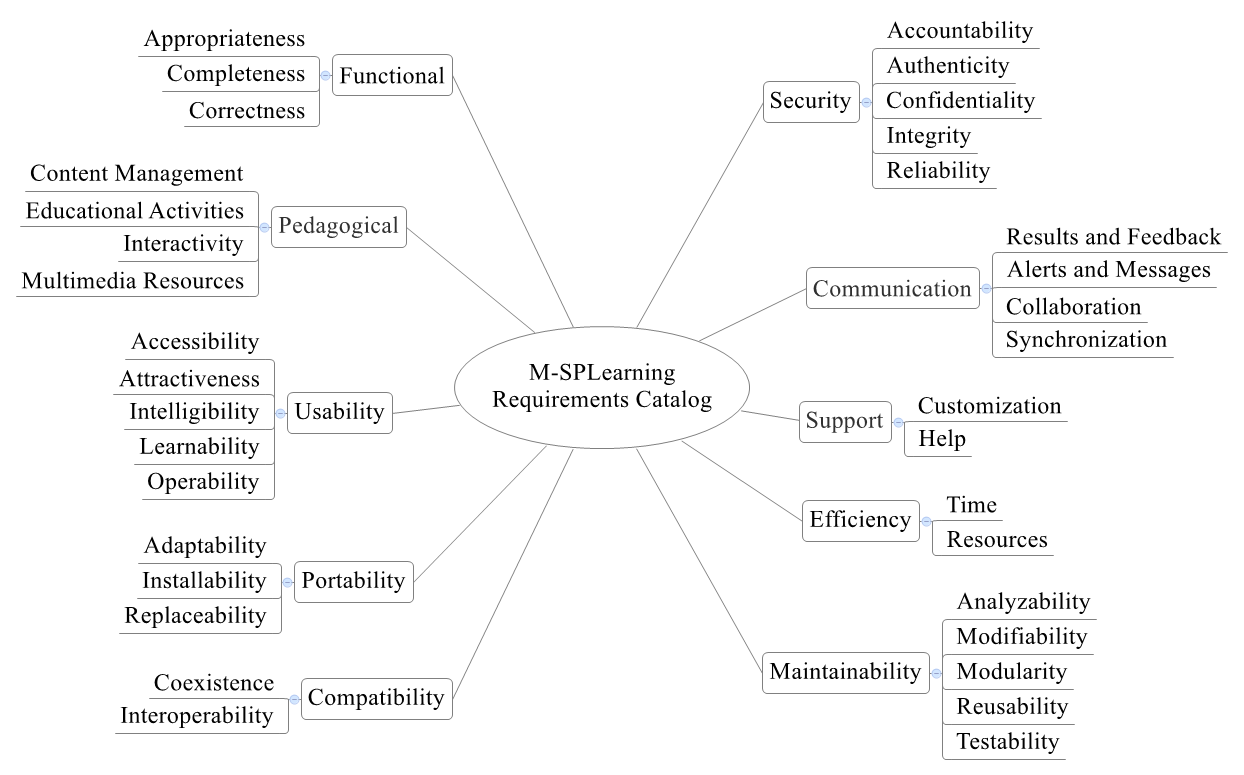
\includegraphics[scale=0.37]{figures/section3/MSPLCatalog}
    \caption{M-SPLear\allowbreak ning Requirements Catalog \protect\cite{falvojr14b}.}
    \label{figureMSPLCatalog}
\end{figure}

%Com base no catálogo de referencia, observou-se que a maioria dos requisitos originalmente propostos eram equivalentes, direta ou indiretamente, às características e subcaracterísticas da norma ISO/IEC 25010. Com isso, acredita-se que a derivação do catálogo forneceu os requisitos educacionais móveis necessários para a concepção da LPS deste trabalho.
According the catalog, most requirements originally proposed were directly or indirectly equivalent to the characteristics and subcharacteristics of ISO/IEC 25010. %Thus, it is believed that the performed  derivation provided us the educational requirements necessary for the M-SPLear\allowbreak ning.
%Em termos estruturais, o catálogo resultante apresentou 10 requisitos primários e 35 secundários. Por exemplo, o elemento Support apresenta características comuns como a internacionalização de mensagens (provida pelo requisito Customization) e ajuda em dúvidas frequentes (Help).
In structural terms, the resulting catalog has 10 primary and 35 secondary requirements. For example, the \textit{Support} element has common features, such as internationalization of messages (provided by \textit{Customization} requirement) and frequently asked questions (\textit{Help}).

%Apesar de possuir requisitos genéricos e aplicáveis a outros domínios, o catálogo proposto também possui características específicas para aplicações m-learning. Por exemplo, a maior parte dos requisitos derivados a partir de Pedagogical e Communication representam necessidades essenciais ao domínio educacional móvel.
Despite it generic requirements, the catalog also has specific features for m-learning applications. For instance, most requirements derived from \textit{Pedagogical} and \textit{Communication} represent essential requirements to the mobile educational domain.

%Em termos pedagógicos, o gerenciamento de conteúdos educativos é fundamental para o desenvolvimento das atividades educacionais. Além disso, a presença de recursos multimédia pode proporcionar acesso a informação de uma forma mais atrativa. Tais peculiaridades sintetizam os requisitos classificados pelo item Pedagogical.
In pedagogical terms, the management of educational content is essential for the development of educational activities. Furthermore, multimedia resources can provide access to information in a more attractive way. Such peculiarities summarize the requirements classified by the \textit{Pedagogical} item.

%Por sua vez, os requisitos provenientes de Comunucation representam funcionalidades relacionadas à troca de mensagens, alertas e o compartilhamento de resultados ou feedbacks, tornando o aprendizado, mais colaborativo e dinâmico. Outra característica importante é a sincronização dos dados de uma aplicação m-learning, pois os usuários podem possuir e utilizar mais de um dispositivo móvel ou plataforma. 
The requirements from \textit{Communication} represent features related to the exchange of messages, alerts and sharing results or feedback, which make the learning process more collaborative and dynamic. Another important feature is the synchronization of data from a mobile learning application, since users can have more than one mobile device or platform.

%A fim de avaliar o catálogo de requisitos proposto para a M-SPLear\allowbreak ning uma validação adicional actividade foi conduzida. Neste sentido, um formulário on-line foi preparado a fim de verificar informalmente as principais questões técnicas relacionadas ao catálogo. O formulário foi disponibilizado em uma estrutura de checklist, com o objetivo de mensurar a opinião de especialistas na área de engenharia de software.
An additional validation activity was conducted for evaluation of the requirements catalog proposed for the M-SPLear\allowbreak ning. An online form was prepared for informally checking the main technical issues related to the catalog. It was structured as a checklist, with 12 multiple choice questions so that it could measure the specialists opinions in software engineering area.

%O documento contou com 12 questões de múltipla escolha, onde as duas primeiras eram relacionadas à experiência dos participantes nos conceitos de LPS e m-learning. Nesse caso, as opções possíveis foram: Proficiente, Intermediário e Novato. As dez  questões restantes referiam-se ao catálogo de requisitos da M-SPLear\allowbreak ning, por exemplo: O catálogo compreende requisitos adequados ao domínio?. Para essas perguntas as opções: Adequado, Regular e Insatisfatório foram aplicadas.
The first two questions were related to the background of the participants on SPL and m-learning concepts and the options were ``Expert", ``Intermediate" and ``Novice". The ten remaining questions were related to the M-SPLear\allowbreak ning requirements catalog, such as \textit{``Does the catalog comprise appropriate requirements to the domain?"}. The options were ``Adequate", ``Regular" and ``Unsatisfactory".

%Os resultados coletados mostraram que, na visão dos participantes, o catálogo de requisitos está adequado ou regular a todos os itens avaliados. Além disso, nenhuma das questões relacionadas ao catálogo de requisitos da M-SPLear\allowbreak ning foi respondida como insatisfatória. A Tabela \ref{tableMSPLChecklist} sintetiza as avaliações médias obtidas a partir dos 11 formulários de ckecklist submetidos.
The questionnaire was answered by 11 participants and the results showed the requirements catalog was ``Adequate", with a mean of 60.90\%, and was ``Regular", with a mean of 39.10\%, for all items evaluated. Furthermore, none of the questions related to the M-SPLear\allowbreak ning was answered as ``Unsatisfactory". 

%Table \ref{tableMSPLChecklist} summarizes the average ratings obtained.
%
%\begin{table}
%    \caption{M-SPLear\allowbreak ning Requirements Catalog Checklist Summary.}
%    \centering
%    \scriptsize
%    \begin{tabular}{cc}
%        \toprule
%        \textbf{Option} & \textbf{Average Percentage Obtained} \\
%        \midrule
%        Adequate       & 60.90\% \\
%        Regular        & 39.10\% \\
%        Unsatisfactory & 0.00\% \\
%        \bottomrule
%    \end{tabular}
%    \label{tableMSPLChecklist}
%\end{table}

Although preliminary, the informal validation performed was important for the evaluation of set of requirements elicited for M-SPLear\allowbreak ning.

%A próxima etapa da atividade de Análise de Domínio consiste em identificar as variabilidades existentes nos produtos da M-SPLear\allowbreak ning, de acordo com a definição da abordagem proativa. Nesse sentido, as variabilidades representam a forma pela qual os produtos são diferenciados em uma LPS, tornando possível a geração dos produtos específicos suportados pela LPS. Em termos práticos, as variabilidades geralmente são identificadas e representadas através do conceito de features.
The next stage of the Domain Analysis activity was the identification of variabilities in the M-SPLear\allowbreak ning products \cite{krueger02}. Variabilities represent the way in which products are differentiated in an SPL and enable possible the generation of specific products supported by the SPL \cite{vangurp01}. In practical terms, variabilities are generally identified and represented through the features concept \cite{bosch01,kang90}.

%No contexto da M-SPLear\allowbreak ning, o catálogo de requisitos foi analisado, e suas características serviram como base para a criação de um modelo feature em conformidade aos requisitos elicitados (Figura X). A interpretação do modelo de features é simples e segue os conceitos tradicionais idealizados pela abordagem Feature-Oriented Domain Analysis (FODA). Basicamente, cada requisito concreto presente no catálogo M-SPLear\allowbreak ning foi transformado em uma feature primária. Com isso, foram modeladas 16 features obrigatórias e 14 features opcionais.
The requirements catalog was analyzed and its characteristics were used as the basis for the creation of a feature model compliant to the requirements elicited (Figure \ref{figureMSPLFeatureModel}). The interpretation of the feature model is straightforward and follows the traditional concepts conceived by the Feature-Oriented Domain Analysis approach (FODA) \cite{kang90}. Basically, each concrete requirement in M-SPLear\allowbreak ning catalog was mapped as a primary feature. Therefore, 16 mandatory features and 14 optional features were modeled.

%Com relação ao catálogo, alguns dos requisitos elicitados foram considerados muito abstratos ou onipresentes em relação do domínio m-learning e, por isso, não foram transformados em features, são eles: (i) Functional; (ii) Portability; (iii) Efficiency; e (iv) Maintainability. Por outro lado, as features primárias e suas respectivas responsabilidades no domínio das aplicações m-learning são apresentadas a seguir, sintetizando as contribuições relacionadas à Análise de Domínio:
Some of the elicited requirements of the catalog were considered too abstract or ubiquitous over the m-learning domain and were not mapped (\textit{Functional}, \textit{Portability}, \textit{Efficiency}, \textit{Maintainability}). The primary features and their responsibilities for m-learning applications are the following:

\begin{itemize}

    %Incorpora requisitos educacionais e pedagógicos, provendo as principais características presentes em aplicações m-learning para atividades de ensino e treinamento. A subfeature Interactivity é opcional, uma vez que está relacionada a interatividade por meio de redes sociais. As subfeatures Content Management, Educational Activities e Multimedia Resources são obrigatórias, onde a última delas possibilita a escolha de um ou mais recursos multimédia como apoio ao ensino.
    \item \textit{Pedagogical}: incorporate educational and pedagogical requirements, providing the main characteristics of m-learning applications for teaching and training activities. Subfeature \textit{Interactivity} is optional, as it is related to interactivity through social networks. Subfeatures \textit{Content Management}, \textit{Educational Activities} and \textit{Multimedia Resources} are mandatory and the latter offers a choice of one or more multimedia resources to support teaching.
    
    %Apresenta características essenciais no que diz respeito à interface visual de uma aplicação m-learning. Tais características são fundamentais para a aceitação do produto no mercado. Essa feature e suas variações determinam que todos os produtos gerados pela LPS devem ter um padrão de usabilidade, provendo qualidade aos usuários finais. Com isso, todas as features em questão foram definidas como obrigatórias.
    %A plataforma Android possui diversas imposições em termos de usabilidade, com o objetivo de padronizar e maximizar a experiência de seus usuários, por este motivo as features em questão foram definidas como abstratas.
    \item \textit{Usability}: address the essential characteristics of the visual interface of a mobile learning application. That are fundamental to the acceptance of the product on the market. All products generated by an SPL must adopt a standard of usability to provide quality to final users, therefore, all features were defined as mandatory.


\begin{figure}
    \centering
    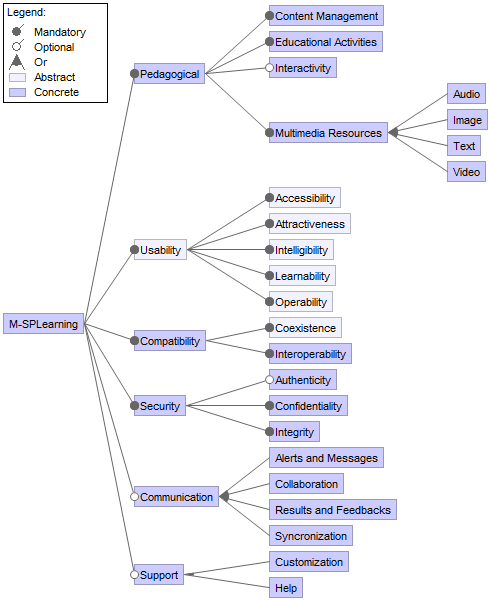
\includegraphics[scale=0.9]{figures/section3/MSPLFeatureModel}
    \caption{M-SPLear\allowbreak ning Feature Model \protect\cite{falvojr14a,falvojr14b}.}
    \label{figureMSPLFeatureModel}
\end{figure}

    %Engloba a coexistência e capacidade de trocar informações com outros sistemas no mesmo ambiente operacional. Por se mostrar essencial a aplicativos móveis, essas features foram definidas como obrigatórias.
    \item \textit{Compatibility}: include the coexistence and ability of a product to exchange information with other systems in a same operating environment. As they are essential for mobile applications, their features were defined as mandatory.
    
    %Trata-se de uma feature fundamental para qualquer aplicativo m-learning, uma vez que existem aspectos que devem ser garantidos para que os usuários confiem no produto gerado. As features que representam a integridade e confidencialidade foram definidas como obrigatórias devido a sua importância em termos de seguraça. Já a feature Authenticity é opcional porque nem todo aplicativo m-learning possui autenticação explícita de seus usuários.
    \item \textit{Security}: this is a key feature since any mobile application should send and receive data securely. Features \textit{Integrity} and \textit{Confidentiality} were defined as mandatory due to their importance in security terms. On the other hand, the \textit{Authenticity} feature is optional because not every m-learning application has explicit authentication of its users.
    
    %Provê o transporte de informações entre os usuários do aplicativo, possibilitando a troca de mensagens, a verificação resultados de testes e até mesmo a sincronização de atividades realizadas em outros dispositivos móveis. Essa feature é opcional e suas subfetaures possuem essa mesma definição, possibilitando qualquer combinação possível entre elas.
    \item \textit{Communication}: responsible for changing information among users of the application, enabling the exchanging of messages, testing results and synchronizing activities in other mobile devices. This feature and subfeatures are optional and accept any possible combinations.
    
    %Trata-se de uma feature considerada um diferencial de qualidade para os produtos em que ela está presente, pois provê alternativas de apoio ao usuário, como ajuda e internacionalização. Foi classificada como opcional por não ser um pré-requisito, assim como suas subfeatures.
    \item \textit{Support}: this feature provides some interesting alternatives to the user, as help and internationalization. All features and subfeatures was classified as an optional because it is not a prerequisite.
\end{itemize}

\subsubsection{Definition of Architecture}

%A partir do modelo de features apresentado anteriormente, definimos uma arquitetura de software aderente às necessidades do domínio educacional móvel. Tal arquitetura e seus respectivos componentes representam de forma abstrata os ativos centrais da M-SPLear\allowbreak ning. Nesse sentido, a maioria das abordagens desenvolvidas para auxiliar no gerenciamento de variabilidades envolvem diversos conceitos e modelos de representação. A abordagem SMarty, em especial, é baseada na UML, amplamente aceita pela comunidade científica. Com isso, devido a sua facilidade de uso e resultados experimentalmente avaliados a SMarty foi escolhida para apoiar esta atividade da M-SPLear\allowbreak ning.
From the feature model is necessary define an adherent software architecture to the mobile domain educational needs. Such an architecture and its components abstractly represent the core assets of M-SPLear\allowbreak ning. Accordingly, most of the approaches developed to assist in the management of variability involve several concepts and representation models. SMarty, in particular, is based on UML, widely accepted by scientific and industrial communities. Due to its ease of use and results (experimentally evaluated), SMarty was chosen to support the design of the M-SPLear\allowbreak ning promising architecture.

%A abordagem SMarty foi essencial durante todo o processo de desenvolvimento da LPS proposta, sobretudo por agregar seu perfil aos modelos UML para representação das similaridades e, principalmente, das variabilidades da M-SPLear\allowbreak ning, como é o caso do diagrama de componentes arquiteturais ilustrado na Figura \ref{figureMSPLArchitecture}. Com base no diagrama arquitetural é possível identificar a base estrutural utilizada para a construção da M-SPLear\allowbreak ning. O pacote com os ativos centrais engloba os componentes que representam as features definidas como concretas no modelo de features.
SMarty played an important role in the development of M-SPLear\allowbreak ning, as it provided standards defined by the SMartyProfile to represent the similarities and, especially, the variabilities of M-SPLear\allowbreak ning. The diagram of architectural components illustrated in Figure \ref{figureMSPLArchitecture} represents one of the diagrams developed with the support of SMarty. Based on the architectural diagram it is possible to identify the structural basis used to the construction of the M-SPLear\allowbreak ning. The package \textit{Core Assets} comprises its concrete features as shown on Figure \ref{figureMSPLFeatureModel}.

\begin{figure}
    \centering
    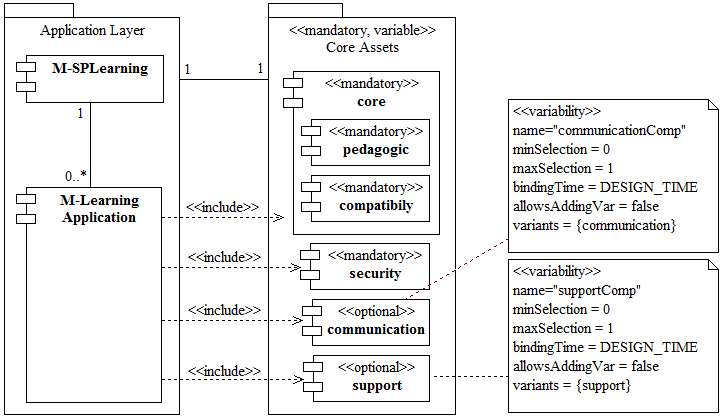
\includegraphics[scale=0.55]{figures/section3/MSPLArchitecture}
    \caption{M-SPLear\allowbreak ning SMarty-based Architecture Diagram.}
    \label{figureMSPLArchitecture}
\end{figure}

%Os componentes que representam features específicas do domínio m-learning foram agrupados e nomeados como core. Assim, foi possível unificar os módulos fundamentais aos produtos gerados através da M-SPLear\allowbreak ning. Além disso, é possível identificar alguns dos elementos da abordagem SMarty, que nesse caso representam as variabilidades em alto nível.
The components that represent the specific features of the m-learning domain were grouped into package \textit{core}. Therefore the fundamental modules for products generated by M-SPLear\allowbreak ning. Could be unified and some of the elements of SMarty, representing the variabilities at a component level.

%A camada de aplicação, por sua vez, contém um componente que caracteriza a M-SPLear\allowbreak ning, identificando sua associação com os ativos centrais e explicitando a possibilidade de criação de produtos, também representados como componentes. Cada produto gerado pode incluir as dependências disponíveis nos ativos centrais, fazendo com que cada produto possa utilizar dependências diferentes de acordo com as configurações definidas na M-SPLear\allowbreak ning.
The \textit{Application Layer} contains a component that characterizes the M-SPLear\allowbreak ning, identifying its association with core assets and enabling products derivation. Each product should include the components available in the \textit{Core Assets}, making each m-learning application has different features according to its configurations defined in M-Learning.

\subsubsection{Components Design}

%Esta fase deve ser conduzida para projetar as variabilidades e similaridades identificadas pela Análise de Domínio. Nesse sentido, os componentes, arquitetonicamente armazenados junto aos ativos centrais, tiveram suas respectivas \textit{features} visualmente representadas por meio de um diagrama de componentes SMarty, ilustrado na Figura \ref{fig:msplDesign}.
In this phase it is designed the variabilities and similarities identified in the Domain Analysis. Accordingly, the core assets elements were visually represented by SMarty diagram components (Figure \ref{figureMSPLDesign}).

\begin{figure}
\centering
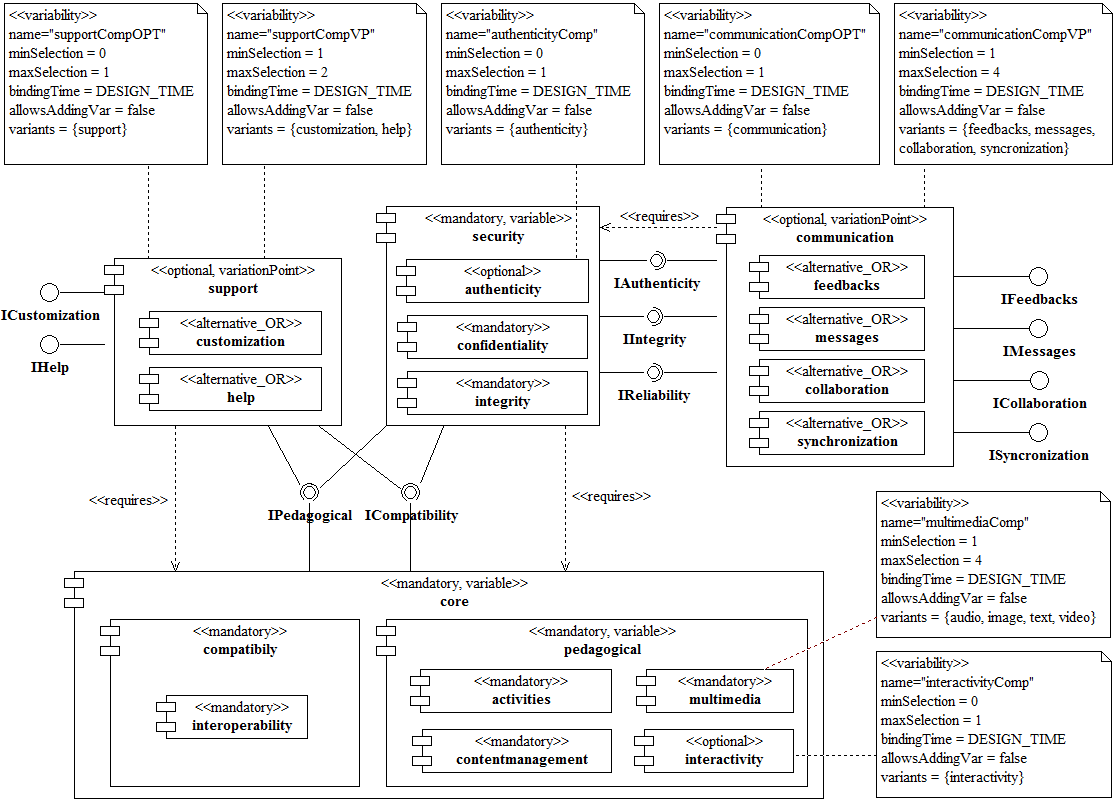
\includegraphics[scale=0.445]{figures/section3/MSPLDesign}
\caption{M-SPLear\allowbreak ning SMarty-based Components Diagram.}
\label{figureMSPLDesign}
\end{figure}

%Por meio desse diagrama de componentes é possível visualizar todas as features concretas contempladas pela M-SPLear\allowbreak ning. Os componentes resultantes foram rotuladas com os estereótipos característicos da abordagem SMarty. Esse diagrama permite a analise da quantidade de configurações possíveis aos aplicativos m-learning contemplados pela LPS.
The diagram shows all concrete features covered by M-SPLear\allowbreak ning. The resulting components are labeled with the characteristic stereotypes of SMarty approach. This diagram presents the possible component configurations, based on features, for m-learning applications covered by the SPL.
%Por exemplo, o componente multimedia foi modelado como uma variabilidade (esteriótipo variability), ou seja, ele pode ser configurado para que uma LPS crie aplicações m-learning customizadas de acordo com suas configurações. Dessa forma, uma aplicação poderia ser configurada para possuir no mínimo um e no máximo quatro recursos multimédia (audio, image, text e video), conforme as notações "minSelection" e "maxSelection". Uma observação relevante é que qualquer componentes cujo filho foi modelado como uma variabilidade deve ser marcado como variável (esteriótipo variable).
For example, the \textit{multimedia} component was modeled with variability stereotype, i.e., the SPL can be configured for creating custom m-learning applications with such features. Therefore, a product can be configured to have between one and four \textit{multimedia} resources (audio, image, text and video), according to notations ``minSelection" and ``maxSelection". Any component formed for other components with variability should be tagged with the variable stereotype.

% 30/12/2015 03:02 %

%Com ênfase no domínio explorado, os componentes pedagogical e communication se destacam, assim como seus requisitos. Nesse sentido, a maioria dos componentes pedagógicos são obrigatórios, com variabilidades possíveis em termos de interatividade e recursos multimídia (já explanada anteriormente). Por sua vez, os componentes agrupados em communication são alternativos, sendo que ao menos um deles deve agregar sua funcionalidade aos produtos gerados.
With emphasis on the explored domain, the \textit{pedagogical} and \textit{communication} components stand out, just like the domain requirements. In this sense, most \textit{pedagogical} subcomponents are mandatory, with possible variabilities in terms of \textit{interactivity} and \textit{multimedia} features, whereas the \textit{communication} subcomponents are alternative, and at least one of them must provide its functionalities to the generated products.

%Também fica explícito o relacionamento de dependência entre os componentes modelados. Como definido anteriormente, o componente core unifica as features integralmente obrigatórias ao domínio m-learning, tornando-se necessário, direta ou indiretamente, aos componentes security, communication e support. A particularidade aqui fica por conta do componente communication, dependente do componente security, que por sua vez está relacionado com o componente core, fazendo com que o componente communication também tenha acesso a essa dependência. Isso garante a imposição arquitetônica de que todos os componentes parcialmente mandatórios ou opcionais dependam do componente core, que proverá as características fundamentais da M-SPLear\allowbreak ning.
The dependency relationship between the modeled components can also be observed. As previously defined, the \textit{core} component unifies the mandatory features for the m-learning domain, being necessary, directly or indirectly, to the \textit{security}, \textit{communication} and \textit{support} components. Particularly, the \textit{communication} component depends on the \textit{security} component, which is related to the \textit{core} component. As a consequence, the \textit{communication} component also knows the \textit{core}.

%A partir do Projeto de Componentes aferidos pela LPS, torna-se possível a definição de um Plano de Produção que transforme as representações abstratas em produtos de software concretos, com suas respectivas variabilidades. A seção a seguir conclui a Análise de Domínio definida para a M-SPLear\allowbreak ning.
Through Components Project it is possible to define a Production Plan to transform the abstract representations in concrete software products, with their respective variabilities, as following.

\subsubsection{Production Plan}

%O Plano de Produção prescreve como os produtos devem ser gerados a partir dos ativos centrais definidos para a LPS. Para isso, um diagrama de atividades usando a abordagem SMarty foi modelado, expondo as variabilidades possíveis durante o processo de criação de um produto (Figura \ref{figureMSPLProductionPlan}). Basicamente, este plano pode ser considerado um ativo central da M-SPLear\allowbreak ning, assim como qualquer outro artefato que contribua para a criação sistemática de seus produtos. 
The Production Plan prescribes how the products should be generated from the core assets identified for the SPL. An activity diagram using the SMarty approach and exposing the possible variabilities in the creation of a product (Figure \ref{figureMSPLProductionPlan}) was modeled. Basically, this plan can be considered a core asset of M-SPLear\allowbreak ning, as any other artifact that contributes to the systematic creation of its products.

\begin{figure}
\centering
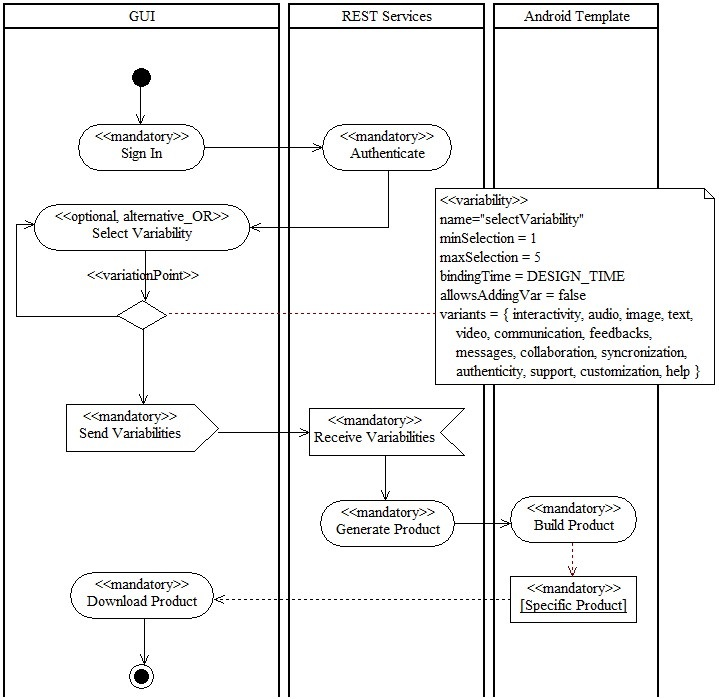
\includegraphics[scale=0.4]{figures/section3/MSPLProductionPlan}
\caption{M-SPLear\allowbreak ning SMarty-based Production Plan.}
\label{figureMSPLProductionPlan}
\end{figure}

%O ponto de variação definido no plano de produção expõe todas as variabilidades elicitadas para a M-SPLear\allowbreak ning. Desta forma, a customização dos produtos foi centralizada em um único ponto, agilizando o processo de configuração e geração dos aplicativos m-learning, provenientes da LPS proposta.
The variation point defined in the production plan exposes all variabilities elicited for M-SPLear\allowbreak ning. Therefore, the customization of the products was centralized at a single point and streamlined the configuration process and generation of m-learning applications by the SPL proposal.

%Cada raia do diagrama representa um módulo específico, sendo possível identificar algumas características arquiteturais da M-SPLear\allowbreak ning. Uma das mais importantes neste sentido é a utilização do conceito de REpresentational State Tranfer (REST). Essa característica permite a criação e consumo de web services por meio do padrão Hypertext Transfer Protocol (HTTP), tornando viável a utilização de arquiteturas emergentes, como a Service-Oriented Architecture (SOA), também no contexto de aplicações móveis.
Each swimlane of the diagram represents a specific module, and enables identification of some architectural characteristics of the M-SPLear\allowbreak ning. One important point is the use of the REpresentational State Transfer (REST) \cite{fielding00} architectural style. Through this concept, web services can be created and consumed by the Hypertext Transfer Protocol (HTTP) and emerging software architectures, as Service-Oriented Architecture (SOA) can be used also in the context of mobile applications.

%A seguir cada módulo representado no diagrama de atividades é sintetizado, considerando suas características técnicas e responsabilidades em termos práticos:
Each module represented in Figure \ref{figureMSPLProductionPlan} is synthesized according to its main characteristics in technical terms:

\begin{itemize}
    %Módulo que provê a interface gráfica dos usuários da LPS, ou seja, as representações visuais com as quais os usuários interagem para a geração dos produtos apoiados pela M-SPLear\allowbreak ning. Neste módulo, é possível configurar as variabilidades e visualizar as similaridades, além de solicitar a geração de um produto personalizado. Este módulo foi implementado utilizando apenas tecnologias client-side, em especial HTML, JavaScript e CSS. A ideia foi demonstrar a interoperabilidade em uma arquitetura SOA, já que foram implementados todos os serviços usando REST, conforme o item a seguir.
	\item \textbf{\textit{Graphical User Interface (GUI):}} a module that provides the visual representations with which users interact to generate the products supported by M-SPLear\allowbreak ning. Variabilities can be configured for the generation of a customized product. This module was implemented through client-side technologies, especially HTML, JavaScript and CSS. The idea was to demonstrate interoperability in a SOA architecture, since all services were implemented using REST.
	
	%Módulo desenvolvido a partir da abstração arquitetônica REST, que se caracteriza pelo uso de tecnologias e protocolos da web para a criação e entrega de serviços. Este estilo é totalmente aderente ao padrão arquitetural SOA e assegura a disponibilidade e consumo de web services de uma forma simples e eficiente. Este módulo corresponde à principal interface entre os produtos gerados pela M-SPLear\allowbreak ning e suas features. Ele acessa um banco de dados remoto, onde todas as informações são armazenadas, incluindo as features (similaridades e variabilidades) especificadas via GUI. A centralização dos dados no módulo de serviços torna-o essencial para os outros (GUI e Android Template), uma vez que ambos consomem os web services disponibilizados por ele.
	\item \textbf{\textit{REST Services:}} a module developed from the REST architectural abstraction and characterized by the use of technologies and protocols of the web for the creation and delivery of services. This style is fully adherent to the SOA architectural pattern and ensures the availability and consumption of web services in a simple and efficient way. It is the main interface between the products generated by the M-SPLear\allowbreak ning and their features and accesses a remote database where all the information is stored, including features (similarities and variabilities) configured from the \textit{GUI}. The centralization of data in the \textit{REST Services} module is essential for other modules (\textit{GUI} and \textit{Android Template}), since both consume the web services provided.
	
	%Este módulo provê um template genérico para a customização dos produtos. Isso permite que um serviço, disponível no módulo REST Services, execute uma compilação personalizada de acordo com as variabilidades configurados no módulo GUI. O resultado é um Android Application Package (APK) com todas as features pré-configuradas, o que permite a instalação do produto customizado em qualquer dispositivo Android.
	\item \textbf{\textit{Android Template:}} a module that provides a generic template for the customization of products. Therefore, the \textit{REST Services} module executes a custom build, according to the variabilities configured in the \textit{GUI}. The result is an Android Application Package (APK) with all pre-configured features for the installation of a custom product on any Android device.
\end{itemize}

%Considerando a necessidade de construção de aplicações m-learning com maior qualidade e reúso, os esforços para o desenvolvimento de LPS que lidam com aspectos SOA ganharam especial importância no contexto móvel. A adoção de uma abordagem SOA torna-se cada vez mais relevante, principalmente porque torna mais fácil e flexível a construção de suas aplicações, promovendo interoperabilidade e reutilização, o que corrobora com as definições arquiteturais propostas no plano de produção.
Considering the need of building m-learning applications with higher quality and reuse, efforts for the development of SPL dealing with SOA aspects gained special importance in the mobile context \cite{marinho10,nascimento11}. The adoption of an SOA approach has become increasingly important, especially because its applications are easy and flexible and promote interoperability and reuse, which agrees with the architectural definitions proposed in the production plan.

%A M-SPLear\allowbreak ning foi elaborada a partir de um processo baseado em práticas e conceitos relevantes no âmbito da Engenharia de Software. Com isso, a M-SPLear\allowbreak ning utilizou um processo sequencial para sua definição, abordando as dificuldades da análise de elementos do domínio e as definições arquiteturais necessárias para sua implementação proativa. A próxima seção trata da atividade primária subsequente, a Engenharia de Aplicação.
M-SPLear\allowbreak ning was elaborated from a process based on relevant practices and concepts in software engineering and has used an incremental process for its definition, addressing the difficulties of domain analysis and the architectural definitions necessary for a proactive implementation. The next section addresses the subsequent SPL activity, i.e., the AE.

\subsection{Application Engineering}\label{section32}

%Esta atividade depende essencialmente dos artefatos de saída da Engenharia de Domínio, que agora atuam como artefatos de entrada. A partir dos ativos gerados, um conjunto específico de features foi selecionado para a implementação da M-SPLear\allowbreak ning. Essa redução de escopo foi definida com o objetivo de viabilizar a avaliação experimental da M-SPLear\allowbreak ning. Dessa forma, com um número reduzido de features, foi possível implementar e avaliar a LPS em um prazo aceitável.
This activity depends on the output artifacts of DE, which now act as input devices. A specific set of features with such artifacts was selected for the implementation of M-SPLear\allowbreak ning. This reduction in scope was defined for an experimental evaluation of the M-SPLear\allowbreak ning. Therefore, the SPL could be implemented with a limited number of features in 188 hours, which enabled their experimental evaluation.

%No contexto deste trabalho, as features relacionadas às atividades pedagógicas e de segurança foram priorizadas e implementadas. O motivo dessa escolha é que as features em questão representam os requisitos funcionais mínimos de uma aplicação m-learning, são eles: (i) Pedagogical: inclui a realização de atividades educacionais através do gerenciamento de conteúdos interativos e recursos multimédia; (ii) Security: agrega em termos de confidencialidade e integridade dos dados, além da possibilidade de autenticação dos usuários; e (iii) Communication: incluiu apenas a feature relacionada à sincronização de dados.
In this study features related to teaching and security activities were prioritized and implemented because they are the minimum functional requirements of an m-learning application: (i) \textit{Pedagogical}: includes educational activities through the management of interactive and multimedia content; (ii) \textit{Security}: provides confidentiality and integrity of data, which includes the user authentication; and (iii) \textit{Communication}: includes features related to data synchronization.

%Tecnicamente, a M-SPLear\allowbreak ning apresenta a visão lógica de uma LPS definida para configuração e geração de aplicações m-learning na plataforma Android. Sua implementação foi feita predominantemente em Java e seu código fonte pode ser consultado a partir do repositório open source GitHub.
In technical terms,  M-SPLear\allowbreak ning shows a logical view of an SPL defined for configuration and generation of m-learning applications on the Android platform. It was implemented predominantly in Java and its source code is available\footnote{http://github.com/falvojr/msplearning} in GitHub open source repository.

%Por definição, a Engenharia de Aplicação instancia os ativos centrais de uma LPS para geração de produtos específicos. Para isso, o plano de produção, até então abstrato, foi utilizado para a construção de seus respectivos módulos concretos. No contexto desta atividade, o módulo GUI foi inevitavelmente o mais explorado, porque todos os produtos são gerados através dele.
By definition, the AE instantiates the core assets of SPL to generate specific products. The production plan was used for the construction of the respective concrete modules. In such an activity, the \textit{GUI} module is inevitably the most exploited, because all products are generated through it.

%A primeira interação entre usuário e a M-SPLear\allowbreak ning ocorre em uma página inicial web. Nela, os usuários podem registrar-se e, posteriormente, autenticar-se na aplicação. Essa interface visual também introduz o domínio e os principais objetivos da M-SPLear\allowbreak ning, contextualizando seus usuários. Outro aspecto relevante foi a construção de suas páginas web completamente baseadas no conceito de layouts responsivos, o que, dentre outras tendências, tornou a representação visual da LPS ainda mais dinâmica e flexível. A Figura \ref{figureMSPLWebLogin} expõe tais características.
The first interaction between the user and M-SPLear\allowbreak ning occurs in a web home page. Users can sign up and access the application. This interface also introduces the domain and the main objectives of M-SPLear\allowbreak ning. Another important aspect refers to the construction of the web pages completely based on the concept of responsive layouts, which makes the visual representation of SPL even more dynamic and flexible. 

%Figure \ref{figureMSPLWebLogin} presents such characteristics.
%
%\begin{figure}
%\centering
%\includegraphics[scale=0.4]{figures/section3/MSPLWebLogin}
%\caption{M-SPLear\allowbreak ning GUI Login.}
%\label{figureMSPLWebLogin}
%\end{figure}

%Com um usuário devidamente autenticado, a interface resultante é a caracterização mais evidente da M-SPLear\allowbreak ning, já que possibilita o gerenciamento visual das variabilidades disponibilizadas pela LPS. Neste ponto, o usuário, por exemplo um professor, simplesmente realiza alguns cliques para geração de um produto específico, criando, assim, um APK com uma aplicação m-learning instalável em qualquer dispositivo Android.
With an authenticated user, the resulting interface represents the M-SPLear\allowbreak ning, as it enables the visual management of all variabilities provided by SPL. At this point, the user, for example a teacher, simply performs a few clicks to generate a specific product that creates an APK that encapsulates a custom m-learning application for any Android device. The page for this procedure is illustrated in Figure \ref{figureMSPLWebGeneration}, which also shows the visual interface for the management of products generated by M-SPLear\allowbreak ning. Furthermore, variabilities related to features prioritized during this implementation can be configured in the products generation.

%A página para a realização desse procedimento é ilustrado pela Figura 1, que também apresenta a interface visual para o gerenciamento dos produtos gerados através da M-SPLear\allowbreak ning. Além disso, é importante observar que as variabilidades relacionadas às features priorizadas durante essa implementação podem ser configuradas na geração dos produtos.

\begin{figure}
\centering
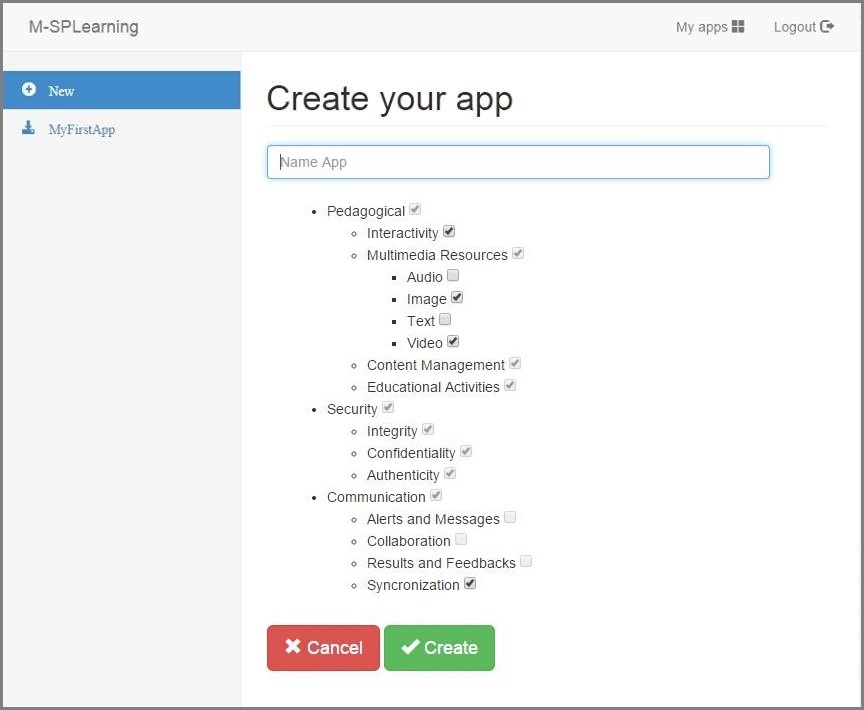
\includegraphics[scale=0.4]{figures/section3/MSPLWebGeneration}
\caption{M-SPLear\allowbreak ning GUI Product Generation.}
\label{figureMSPLWebGeneration}
\end{figure}

%Ao solicitar a geração de um APK, os módulos REST Service e Android Template são acionados simultaneamente. Essa integração resulta na criação de um produto aderente às variabilidades selecionadas pelo usuário. A partir deste momento a aplicação m-learning gerada pode ser instalada no dispositivo móvel de qualquer professor ou aluno, que deve se registrar na aplicação móvel, caso a feature Authentication tenha sido selecionada durante a criação do APK.
When the generation of as APK is required, the \textit{REST Services} and \textit{Android Template} modules are triggered simultaneously. This integration results in the creation of an adherent product for user's selected variabilities. The m-learning application generated can be installed in the Android device of any teacher or student, who must register with the mobile application if feature \textit{Authentication} has been selected in the creation of the APK.

%A Figura 1 mostra dois produtos gerados com as variabilidades Authenticity e Interactivity configuradas de formas diferentes, nas quais: (a) o produto foi configurado apenas com a feature Authenticity; e (b) o produto foi gerado com ambas as variabilidades, o que explica o formulário de autenticação com a possibilidade de interação com algumas redes sociais.
Figure \ref{figureMSPLLogin} shows two products generated with \textit{Authenticity} and \textit{Interactivity} variabilities configured in different ways: (a) the product was configured with only the Authenticity feature; and (b) the product was generated with both variabilities, which explains the authentication form with the possibility of interaction with some social networking.

\begin{figure}
\centering
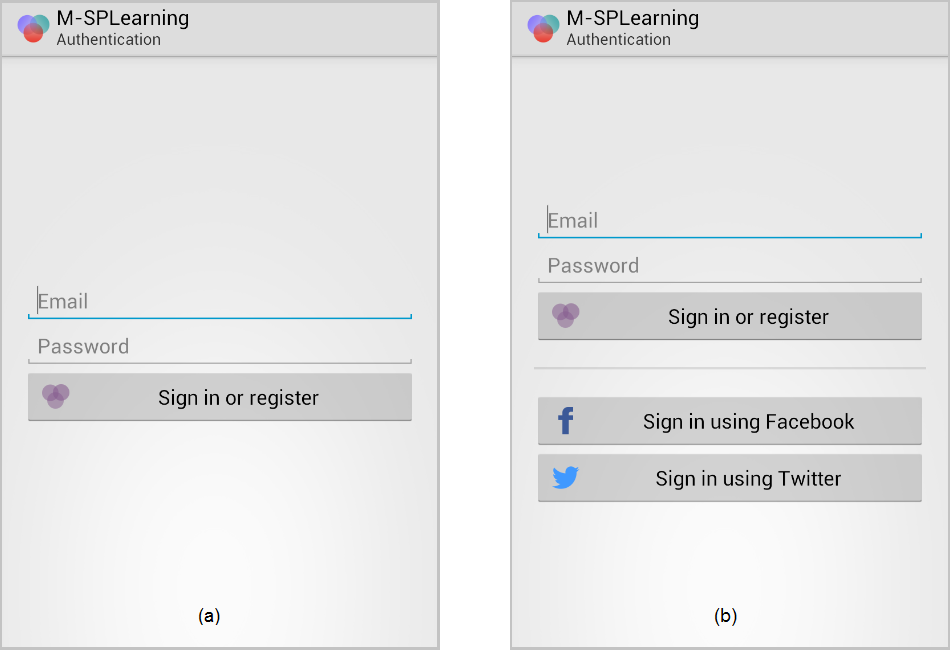
\includegraphics[scale=0.33]{figures/section3/MSPLLogin}
\caption{M-SPLear\allowbreak ning Product Login -- Configurations of the features:\newline(a) \textit{Authenticity}; and (b) \textit{Authenticity} and \textit{Interactivity}.}
\label{figureMSPLLogin}
\end{figure}

%Observando a Figura 1 nota-se que o botão comum aos produtos também prevê a possibilidade de registro de um novo usuário. Para isso, o usuário deve apenas preencher seu e-mail e senha nos campos disponíveis para que a aplicação m-learning verifique a existência de seu usuário. Em caso negativo, o formulário de cadastro é exibido já com as informações digitadas preenchidas (Figura 2).
According to Figure \ref{figureMSPLLogin}, the common button for products also provides the possibility of registering. For this, the user should fill his/her email and password in the fields available for the application to verify if the user exists (Figure \ref{figureMSPLRegister} (a)). If not, the registration form is displayed with the information previously typed (Figure \ref{figureMSPLRegister} (b)).

\begin{figure}
\centering
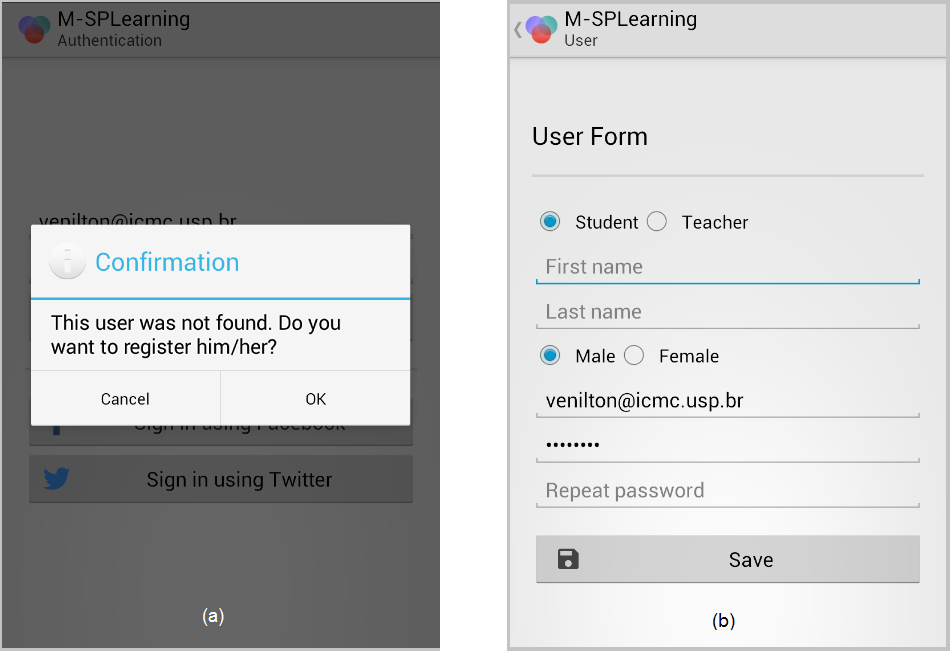
\includegraphics[scale=0.33]{figures/section3/MSPLRegister}
\caption{M-SPLear\allowbreak ning Product Registration -- Steps for user registration:\newline(a) Confirmation message; and (b) Registration Form.}
\label{figureMSPLRegister}
\vspace{0.65cm}
\end{figure}

%O formulário de cadastro de usuário permite a seleção do tipo de acesso: professor ou aluno. Por motivos de segurança, todos os usuários registrados devem ser aprovados pelo usuário que gerou o APK. Para isso, no momento de criação da aplicação o usuário é associado a mesma com perfil administrativo. Esse aspecto deixa evidente a feature "Content Management", uma vez que cada perfil de usuário prevê acessos específicos e bem definidos. A Figura 1 ilustra um cenário possível, em que: (a) apresenta a visão de um professor; e (b) apresenta a visão de um aluno, com o adendo de que neste exemplo nenhum conteúdo educacional foi incluído, tendo em vista que o acesso a esta funcionalidade está desabilitado.
A user can select the type of access, teacher or student in the registration form. For security reasons, all registered users must be approved by the user who generated the APK. At the time of the APK creation the user is associated with an administrative profile. This aspect clarifies feature \textit{Content Management}, since each user's profile provides specific and well-defined accesses. Figure \ref{figureMSPLDashboardApp} illustrates a possible scenario with (a) teacher's views and (b) student's view, but with no content, since the access to this feature is disabled.

\begin{figure}
\centering
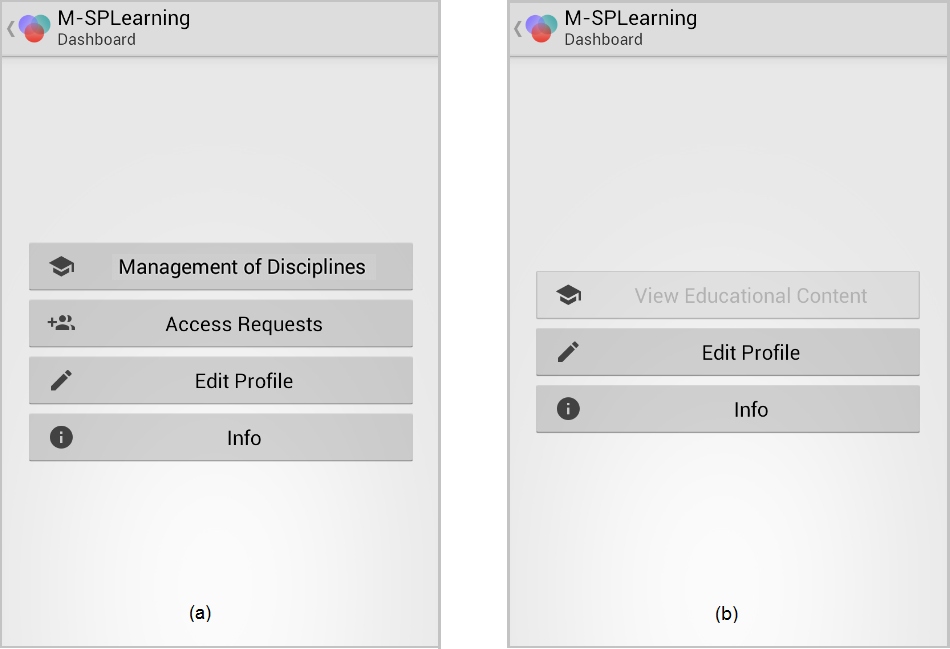
\includegraphics[scale=0.34]{figures/section3/MSPLDashboardApp}
\caption{M-SPLear\allowbreak ning Product Dashboard -- Access Profiles:\newline(a) Teacher; and (b) Student.}
\label{figureMSPLDashboardApp}
\end{figure}

%Com um usuário devidamente autenticado e com suas respectivas funcionalidades fornecidas, a aplicação m-learning está pronta para armazenamento e compartilhamento do seu principal ativo, os conteúdos educacionais. Neste sentido, o professor pode cadastrar suas disciplinas, lições e finalmente o conteúdo de cada uma delas. Essas funcionalidades representam um contexto de uso das features Educational Activities e Multimedia Resources, também representadas pela Figura 1.
After the user has been properly authenticated, the m-learning application is ready for storage and sharing of its main asset, i.e., the educational content. The teacher can register his/her courses, lessons and finally the content of each lesson. These functionalities are a usage sample of the \textit{Educational Activities} and \textit{Multimedia Resources} shown in Figure \ref{figureMSPLEducationalContent}.

\begin{figure}
\centering
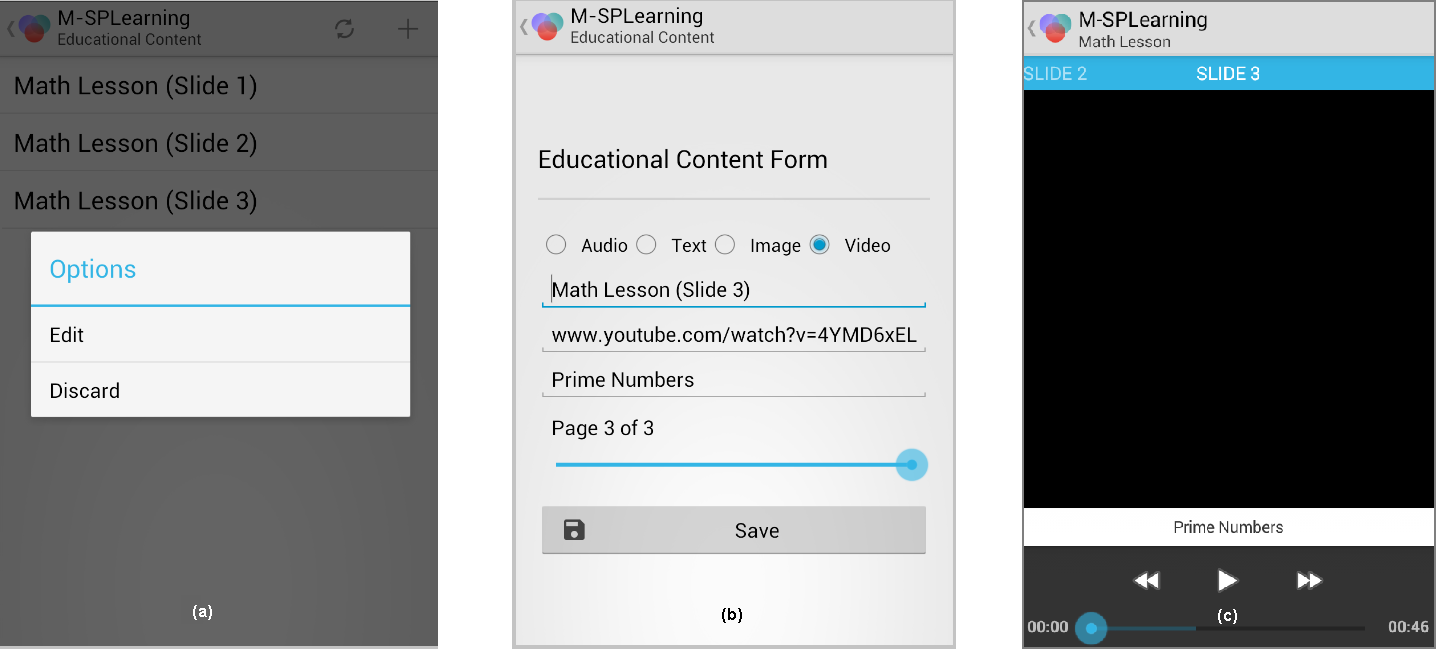
\includegraphics[scale=0.34]{figures/section3/MSPLEducationalContent}
\caption{M-SPLear\allowbreak ning Product Educational Content Management:\newline(a) Listing of educational content and context menu; (b) Editing form; and (c) Displaying video content.}
\label{figureMSPLEducationalContent}
\end{figure}

%De acordo com as features disponibilizadas pela M-SPLear\allowbreak ning, nota-se a possibilidade de inclusão de conteúdos educacionais dos seguintes tipos: áudio, texto, imagem e vídeo. No exemplo apresentado, a opção de vídeo está selecionada, o que provê ao professor a inclusão de uma URL para a disponibilização do vídeo desejado aos alunos que compartilham essa aplicação.
According to the features provided by M-SPLear\allowbreak ning as audio, text, image and video can be included. %In the example shown, the video is selected, providing to the teacher the inclusion of an URL to the availability of the desired video students to share this application.
%Assim, os alunos visualizam os conteúdos educacionais incluídos pelos professores cadastrados na aplicação, obtendo assim acesso centralizado a sua gama de conteúdos educacionais. A Figura 1 ilustra, na perspectiva de aluno, um exemplo de conteúdo educacional do tipo vídeo.
Figure \ref{figureMSPLEducationalContent} (c) illustrates an example of a video feature from a student perspective.

%É importante observar que foi possível incluir os requisitos previamente definidos para a construção de uma LPS. A concepção da M-SPLear\allowbreak ning envolveu desde a análise e projeto até a implementação funcional da proposta desta pesquisa. A avaliação formal da M-SPLear\allowbreak ning, junto de sua abordagem e principais resultados, são descritos na Seção \ref{section4}.
The requirements previously set for the construction of an SPL can also be included. The design of the M-SPLear\allowbreak ning involved from analysis and design to functional implementation. A formal evaluation of the M-SPLear\allowbreak ning, along with this approach and main results is described in Section \ref{section4}.